% CS.tex
\chapter{Cubed-Sphere}

La sphère $\mathbb{S}_a^2$ est couverte de six panels notés (I), ..., (VI). Pour chacun de ces panels il est possible d'associer des angles qui localisent un point ainsi que des bases covariantes et contravariantes qui permettent de calculer les opérateurs différentiels classiques.

\section{Localisation des points et bases}

Sur chaque panel on peut localiser un point grâce à un ensemble d'angles. De plus, une base de vecteur est donnée pour l'espace $\mathbb{T}\mathbb{S}_a^2$. Dans cette partie, on considère les points Nord : $N (0,0,a)$, Sud: $S (0,0,-a)$, Est: $E (0,a,0)$,Ouest: $W (0,-a,0)$, Front: $F(a,0,0)$ et Bottom: $B(-a,0,0)$. 

\subsection{Panel I}

On note $C_0^{(1)}$ le grand cercle à la surface de la sphère $\mathbb{S}_a^2$ passant par les points $N$ et $S$ et contenu dans le plan $(yOz)$. Le cercle $C_0^{(2)}$ est une rotation de ce cercle. Il passe par $E$ et $W$ et est contenu dans le plan $(xOy)$.

Dès lors, on note $C_{\xi}^{(1)}$ le cercle obtenu par rotation de $C_0^{(1)}$ d'un angle $\xi$ autour de l'axe $(Oz)$ (égal à l'axe $(NS)$). $C_{\eta}^{(2)}$ le cercle obtenu par rotation de $C_0^{(2)}$ d'un angle $\eta$ autour de l'axe $(Ox)$ (égal à l'axe $(EW)$). $\xi$ est compté positivement vers les $y$ positifs et $\eta$ positivement vers les $z$ positifs.

Un point $\mathbf{x} \in \mathbb{S}_a^2$ est situé à l'intersection de deux de ces cercles : $\mathbf{x} \in C_{\xi}^{(1)} \cap C_{\eta}^{(2)}$. On note $\alpha$ l'absisse curviligne de $\mathbf{x}$ le long de $C_{\eta}^{(2)}$ avec $C_{0}^{(1)}\cap C_{\eta}^{(2)}$ comme origine. $\beta$ est l'absisse curviligne de $\mathbf{x}$ le long de $C_{\xi}^{(1)}$ avec $C_{0}^{(2)}\cap C_{\xi}^{(1)}$ comme origine (voir Figure \ref{fig:coord cs}). 

\begin{figure}
\begin{center}
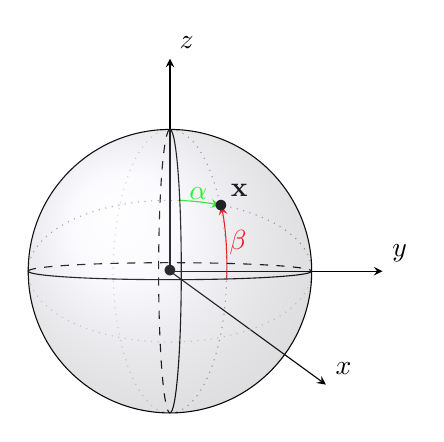
\begin{tikzpicture}[scale=1.8]
	\draw (0,0) node {$\bullet$} ;
	\draw [>=stealth, ->] (0,0) -- (1.5,0) ; 
	\draw (1.5,0) node[above right]{$y$} ;   
	\draw [>=stealth, ->] (0,0) -- (1.1,-0.8) ; 
	\draw (1.1,-0.8) node[above right]{$x$} ; 
	\draw [>=stealth, ->] (0,0) -- (0,1.5) ; 
	\draw (0,1.5) node[above right]{$z$} ; 

    \draw[>=stealth, ->,color=green] (0.065,0.5) arc (85:68:1cm and 0.5cm);
    \draw[color=green] (0.2,0.55) node{$\alpha$} ;
    \draw[>=stealth, ->,color=red] (0.4,-0.05) arc (-5:25:0.41cm and 1cm);
    \draw[color=red] (0.48,0.2) node{$\beta$} ;
    \draw (-1,0)[dotted, color=black!40] arc (180:360:1cm and -0.5cm);
    \draw (0,1)[dotted, color=black!40] arc (90:270:-0.4cm and 1cm);
    \draw (-1,0)[dotted, color=black!20] arc (180:360:1cm and 0.5cm);
    \draw (0,1)[dotted, color=black!20] arc (90:270:0.4cm and 1cm);
    
    \draw (-1,0) arc (180:360:1cm and 0.06cm);
    \draw (0,1) arc (90:270:-0.08cm and 1cm);
    \draw[dashed] (-1,0) arc (180:360:1cm and -0.06cm);
    \draw[dashed] (0,1) arc (90:270:0.08cm and 1cm);
    
    \draw (0.36,0.46) node {$\bullet$} ;
	\draw (0.36,0.46) node[above right]{$\mathbf{x}$} ;
    \draw (0,0) circle (1cm);
    \shade[ball color=blue!10!white,opacity=0.20] (0,0) circle (1cm);
\end{tikzpicture}
\hspace{2cm}
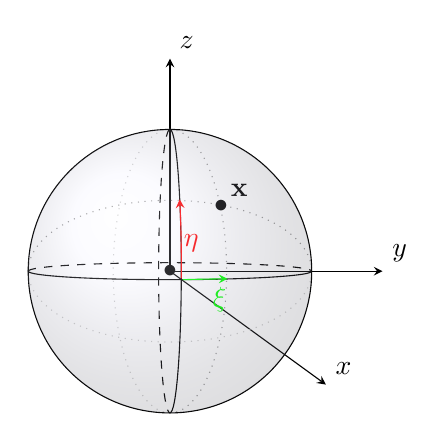
\begin{tikzpicture}[scale=1.8]
	\draw (0,0) node {$\bullet$} ;
	\draw [>=stealth, ->] (0,0) -- (1.5,0) ; 
	\draw (1.5,0) node[above right]{$y$} ;   
	\draw [>=stealth, ->] (0,0) -- (1.1,-0.8) ; 
	\draw (1.1,-0.8) node[above right]{$x$} ; 
	\draw [>=stealth, ->] (0,0) -- (0,1.5) ; 
	\draw (0,1.5) node[above right]{$z$} ; 
    
    \draw (-1,0)[dotted, color=black!40] arc (180:360:1cm and -0.5cm);
    \draw (0,1)[dotted, color=black!40] arc (90:270:-0.4cm and 1cm);
    \draw (-1,0)[dotted, color=black!20] arc (180:360:1cm and 0.5cm);
    \draw (0,1)[dotted, color=black!20] arc (90:270:0.4cm and 1cm);
    
    \draw (-1,0) arc (180:360:1cm and 0.06cm);
    \draw (0,1) arc (90:270:-0.08cm and 1cm);
    \draw[dashed] (-1,0) arc (180:360:1cm and -0.06cm);
    \draw[dashed] (0,1) arc (90:270:0.08cm and 1cm);
    
    \draw[>=stealth, ->,color=green] (0.09,-0.06) arc (225:247:1cm and -0.03cm);
    \draw[color=green] (0.35,-0.2) node{$\xi$} ;
    \draw[>=stealth, ->,color=red] (0.08,-0.05) arc (-5:28:0.1cm and 1cm);
    \draw[color=red] (0.15,0.2) node{$\eta$} ;
    
    \draw (0.36,0.46) node {$\bullet$} ;
	\draw (0.36,0.46) node[above right]{$\mathbf{x}$} ;
    \draw (0,0) circle (1cm);
    \shade[ball color=blue!10!white,opacity=0.20] (0,0) circle (1cm);
\end{tikzpicture}
\caption{Angles $(\alpha, \beta)$ (gauche) et $(\xi,\eta)$ (droite) associés au panel (I) de la Cubed-Sphere}
\label{fig:coord cs}
\end{center}
\end{figure}


\begin{definition}
On nomme panel I l'ensemble des points $\mathbf{x}=(x,y,z)$ de $\mathbb{S}_a^2$ vérifiant $x>0$ et tels que si $\mathbf{x} \in C_{\xi}^{(1)} \cap C_{\eta}^{(2)}$ alors $-\frac{\pi}{4}\leq \xi,\eta \leq \frac{\pi}{4}$. Avec les $\xi$ et $\eta$ associés respectivement aux axes $(NS)$ et $(EW)$. Lorsque $-\pi \leq \xi,\eta \leq \pi$, on parle de Panel I étendu.
\end{definition}

Un point $\mathbf{x}$ du panel I est localisé grâce aux coordonnées cartésiennes $(x,y,z)$ dans $\mathbb{R}^3$ mais aussi en utilisant les paires d'angles $(\alpha, \eta)$ ou $(\xi, \beta)$. Le lien peut-être fait grâce aux égalités suivantes :

\begin{equation}
\left\lbrace
\begin{array}{rcccc}
x & = & a \cos \alpha \cos \eta & = & a \cos \beta \cos \xi \\
y & = & a \sin \alpha & = & a \cos \beta \sin \xi \\
z & = & a \cos \alpha \sin \eta & = & a \sin \beta \\
\end{array}
\right.
\end{equation}

Les coordonnées gnomoniques sont données par $(X,Y)$ :

\begin{equation}
X=\dfrac{y}{x}=\tan \xi \hspace{1cm} Y = \dfrac{z}{x} = \tan \eta
\end{equation}

$x^2+y^2=a^2 \cos^2 \alpha$, donc :

\begin{equation}
\tan^2 \alpha = \dfrac{y^2}{x^2+z^2} = \dfrac{X^2}{1+Y^2}
\end{equation}

de même :

\begin{equation}
\tan^2 \beta = \dfrac{z^2}{x^2+y^2} = \dfrac{Y^2}{1+X^2}
\end{equation}

On en déduit les relations liant $\xi$, $\eta$, $\alpha$ et $\beta$ :

\begin{equation}
\left\lbrace
\begin{array}{rcl}
\alpha & = & \arctan \left( \dfrac{X}{\sqrt{1+Y^2}} \right)\\
\beta & = & \arctan \left( \dfrac{Y}{\sqrt{1+X^2}} \right)
\end{array}
\right.
\label{eq: alpha(xi) beta(eta)}
\end{equation}

et en dérivant et en notant $\delta=\sqrt{1+X^2+Y^2}$ :

\begin{equation}
\dfrac{\partial \alpha}{\partial \xi} = \cos \eta \dfrac{1+X^2}{1+\cos^2 \eta X^2} = \dfrac{1+X^2}{ \delta^2 \cos \eta}\hspace{1cm} \dfrac{\partial \beta}{\partial \eta} = \cos \xi \dfrac{1+Y^2}{1+\cos^2 \xi Y^2}= \dfrac{1+Y^2}{ \delta^2 \cos \xi }
\label{eq; der alpha beta}
\end{equation}

La base locale $(\mathbf{g}_{\xi}, \mathbf{g}_{\eta})$ associée à $(\xi,\eta)$ est donnée par :

$$\mathbf{g}_{\xi} = \dfrac{\partial \mathbf{x}}{\partial \xi} \hspace{1cm} \mathbf{g}_{\eta} = \dfrac{\partial \mathbf{x}}{\partial \eta}.$$

Ainsi, en posant $\delta = \sqrt{1+X^2+Y^2}$, $\mathbf{g}_{\xi}$ et $\mathbf{g}_{\eta}$ sont donnés par :

\begin{equation}
\mathbf{g}_{\xi} = \dfrac{1+X^2}{\delta^2} \begin{pmatrix}
-y \\ x(1+Y^2) \\ -yY
\end{pmatrix} \text{ et } \mathbf{g}_{\eta} = \dfrac{1+Y^2}{\delta^2} \begin{pmatrix}
-z \\ -zX \\ x(1+X^2)
\end{pmatrix}
\label{eq: base locale I}
\end{equation}


Pour tenir compte de la non-orthogonalité des coordonnées, il considérer la métrique pour le calcul des opérateurs et de la base duale.

Le tenseur métrique est donné par :

\begin{equation}
\mathbf{G} = \begin{pmatrix}
\mathbf{g}_{\xi} \cdot \mathbf{g}_{\xi} & \mathbf{g}_{\xi} \cdot \mathbf{g}_{\eta} \\
\mathbf{g}_{\eta} \cdot \mathbf{g}_{\xi} & \mathbf{g}_{\eta} \cdot \mathbf{g}_{\eta}
\end{pmatrix}
\label{eq: metrique}
\end{equation}

Ainsi, après calcul, on a :

\begin{equation}
\mathbf{G} = \begin{pmatrix}
G_{1,1} & G_{1,2} \\ G_{2,1} & G_{2,2}
\end{pmatrix} = a^2 \dfrac{(1+X^2)(1+Y^2)}{\delta^4} \begin{pmatrix}
1+X^2 & -XY \\ -XY & 1+Y^2
\end{pmatrix}
\end{equation}

que l'on peut inverser en :

\begin{equation}
\mathbf{G}^{-1} = \begin{pmatrix}
G^{1,1} & G^{1,2} \\ G^{2,1} & G^{2,2}
\end{pmatrix} = \dfrac{\delta^2}{a^2 (1+X^2)(1+Y^2)} \begin{pmatrix}
1+Y^2 & XY \\ XY & 1+X^2
\end{pmatrix}
\label{eq: metrique inverse}
\end{equation}

On cherche la base $(\mathbf{g}_{\xi},\mathbf{g}_{\eta})$ obtenue par dualité :

\begin{equation}
\left\lbrace
\begin{array}{rcccl}
\mathbf{g}_{\xi} \cdot \mathbf{g}^{\xi} & = & \mathbf{g}_{\eta} \cdot \mathbf{g}^{\eta} & = & 1 \\
\mathbf{g}_{\xi} \cdot \mathbf{g}^{\eta} & = & \mathbf{g}_{\eta} \cdot \mathbf{g}^{\xi} & = & 0 \\
\end{array}
\right.
\end{equation}

d'où la relation suivante :

\begin{equation}
\left\lbrace
\begin{array}{rcl}
\mathbf{g}^{\xi} & = & G^{1,1} \mathbf{g}_{\xi} + G^{1,2} \mathbf{g}_{\eta} \\
\mathbf{g}^{\eta} & = & G^{2,1} \mathbf{g}_{\xi} + G^{2,2} \mathbf{g}_{\eta} \\
\end{array}
\right.
\end{equation}

ainsi, on peut calculer :

\begin{equation}
\mathbf{g}^{\xi} = \dfrac{1}{x(1+X^2)}\begin{pmatrix}
-X \\ 1 \\ 0
\end{pmatrix} \text{ et } \mathbf{g}^{\eta} = \dfrac{1}{x(1+Y^2)}\begin{pmatrix}
-Y \\ 0 \\ 1
\end{pmatrix}
\label{eq: base duale I}
\end{equation}

$( \mathbf{g}^{\xi}, \mathbf{g}^{\eta})$ est la base duale de $(\mathbf{g}_{\xi}, \mathbf{g}_{\eta})$ par rapport à la métrique $\mathbf{G}$.

\begin{remarque}
Lorsque cela portera à confusion, on notera $\mathbf{g}_{\xi}^{(K)}$, $\mathbf{g}_{\eta}^{(K)}$ ainsi que $\mathbf{g}^{(K),\xi}$ et $\mathbf{g}^{(K),\eta}$ où $K$ note le panel concerné $K \in \lbrace I, II, III, IV, V, VI \rbrace$. Dans cette sous-section par exemple $K=I$.   
\end{remarque}






\subsection{Panel II}

On construit le panel II de manière similaire en partant de cercles passants par $N$ et $S$ pour les $C_{\xi}^{(1)}$ ($C_{0}^{(1)}$ est contenu dans le plan $(yOz)$) et les cercles $C_{\eta}^{(2)}$ passant par les points $F$ et $B$ ($C_{0}^{(2)}$ est contenu dans le plan $(xOy)$). Les angles $\xi$, $\eta$, $\alpha$ et $\beta$ sont construits comme précédemment.  $\xi$ est compté positivement lorsque $x$ est négatifs et $\eta$ positivement lorsque $z$ est positifs.

\begin{definition}
On nomme panel II l'ensemble des points $\mathbf{x}=(x,y,z)$ de $\mathbb{S}_a^2$ vérifiant $y>0$ et tels que si $\mathbf{x} \in C_{\xi}^{(1)} \cap C_{\eta}^{(2)}$ alors $-\frac{\pi}{4}\leq \xi,\eta \leq \frac{\pi}{4}$. Avec les $\xi$ et $\eta$ associés respectivement aux axes $(NS)$ et $(FB)$. Lorsque $-\pi \leq \xi,\eta \leq \pi$, on parle de Panel II étendu.
\end{definition}

Un point $\mathbf{x}=(x,y,z)$ du panel II a ses coordonnées qui vérifient la relation suivante :

\begin{equation}
\left\lbrace
\begin{array}{rcccc}
x & = & - a \sin \alpha & = & - a \cos \beta \sin \xi \\
y & = & a \cos \alpha \cos \eta & = & a \cos \beta \cos \xi \\
z & = & a \cos \alpha \sin \eta & = & a \sin \beta
\end{array}
\right.
\end{equation}

Les coordonnées gnomoniques sont données par :

\begin{equation}
X = \tan \xi = - \dfrac{x}{y} \hspace{1cm} Y = \tan \eta = \dfrac{z}{y}
\end{equation}

les relations concernant $\alpha$ et $\beta$ (\eqref{eq: alpha(xi) beta(eta)} et \eqref{eq; der alpha beta}) sont toujours vérifiées, ainsi que celles sur la métrique \eqref{eq: metrique} et \eqref{eq: metrique inverse}.

Ainsi, on peut écrire : 

\begin{equation}
\mathbf{g}_{\xi} = \dfrac{1+X^2}{\delta^2} \begin{pmatrix}
-y(1+Y^2) \\ x \\ xY
\end{pmatrix} \text{ et } \mathbf{g}_{\eta} = \dfrac{1+Y^2}{\delta^2} \begin{pmatrix}
zX \\ -z \\ y(1+X^2)
\end{pmatrix}
\label{eq: base locale II}
\end{equation}

et la base dual par rapport à la métrique :

\begin{equation}
\mathbf{g}^{\xi} = \dfrac{1}{y(1+X^2)}\begin{pmatrix}
-1 \\ -X \\ 0
\end{pmatrix} \text{ et } \mathbf{g}^{\eta} = \dfrac{1}{y(1+Y^2)}\begin{pmatrix}
0 \\ -Y \\ 1
\end{pmatrix}
\label{eq: base duale II}
\end{equation}














\subsection{Panel III}

Le panel III est construit à partir de cercles passants par $N$ et $S$ pour les $C_{\xi}^{(1)}$ ($C_{0}^{(1)}$ est contenu dans le plan $(xOz)$) et les cercles $C_{\eta}^{(2)}$ passant par les points $E$ et $W$ ($C_{0}^{(2)}$ est contenu dans le plan $(xOy)$). Les angles $\xi$, $\eta$, $\alpha$ et $\beta$ sont construits comme dans le panel I. $\xi$ croit en même temps que $-y$ et $\eta$ positivement lorsqu'il croit en même temps que $z$.

\begin{definition}
On nomme panel III l'ensemble des points $\mathbf{x}=(x,y,z)$ de $\mathbb{S}_a^2$ vérifiant $x<0$ et tels que si $\mathbf{x} \in C_{\xi}^{(1)} \cap C_{\eta}^{(2)}$ alors $-\frac{\pi}{4}\leq \xi,\eta \leq \frac{\pi}{4}$. Avec les $\xi$ et $\eta$ associés respectivement aux axes $(NS)$ et $(EW)$. Lorsque $-\pi \leq \xi,\eta \leq \pi$, on parle de Panel IIII étendu.
\end{definition}

Un point $\mathbf{x}=(x,y,z)$ du panel III a ses coordonnées qui vérifient la relation suivante :

\begin{equation}
\left\lbrace
\begin{array}{rcccc}
x & = & - a \cos \alpha \cos \eta & = & a \cos \beta \cos \xi \\
y & = & - a \sin \alpha & = & - a \cos \beta \sin \xi \\
z & = & a \cos \alpha \sin \eta & = & a \sin \beta
\end{array}
\right.
\end{equation}

Les coordonnées gnomoniques sont données par :

\begin{equation}
X = \tan \xi = - \dfrac{y}{x} \hspace{1cm} Y = \tan \eta = \dfrac{z}{x}
\end{equation}

Les équations (\ref{eq: alpha(xi) beta(eta)}, \ref{eq; der alpha beta}, \ref{eq: metrique}, \ref{eq: metrique inverse}) restent vraies. 

Une base locale est :

\begin{equation}
\mathbf{g}_{\xi} = \dfrac{1+X^2}{\delta^2} \begin{pmatrix}
-y \\ x(1+Y^2) \\ yY
\end{pmatrix} \text{ et } \mathbf{g}_{\eta} = \dfrac{1+Y^2}{\delta^2} \begin{pmatrix}
-z \\ -zX \\ x(1+X^2)
\end{pmatrix}
\label{eq: base locale III}
\end{equation}

La base duale de \eqref{eq: base locale III} par rapport à la métrique $\mathbf{G}$ est :

\begin{equation}
\mathbf{g}^{\xi} = \dfrac{1}{x(1+X^2)}\begin{pmatrix}
-X \\ 1 \\ 0
\end{pmatrix} \text{ et } \mathbf{g}^{\eta} = \dfrac{1}{x(1+Y^2)}\begin{pmatrix}
-Y \\ 0 \\ -1
\end{pmatrix}
\label{eq: base duale III}
\end{equation}
















\subsection{Panel IV}

Le panel IV est le symétrique du panel II. On utilise un réseau cercles passants par $N$ et $S$ pour les $C_{\xi}^{(1)}$ ($C_{0}^{(1)}$ est contenu dans le plan $(yOz)$) et les cercles $C_{\eta}^{(2)}$ passant par les points $F$ et $B$ ($C_{0}^{(2)}$ est contenu dans le plan $(xOy)$). Les angles $\xi$, $\eta$, $\alpha$ et $\beta$ sont construits comme dans le panel I. $\xi$ et $x$ croissent en même temps, de même pour $\eta$ et $z$. Le panel IV est constitué d'un ensemble de points symétriques avec le panel II.

\begin{definition}
On nomme panel IV l'ensemble des points $\mathbf{x}=(x,y,z)$ de $\mathbf{S}_a^2$ vérifiant $y<0$ et tels que si $\mathbf{x} \in C_{\xi}^{(1)} \cap C_{\eta}^{(2)}$ alors $-\frac{\pi}{4}\leq \xi,\eta \leq \frac{\pi}{4}$. Avec les $\xi$ et $\eta$ associés respectivement aux axes $(NS)$ et $(FB)$. Lorsque $-\pi \leq \xi,\eta \leq \pi$, on parle de Panel IV étendu.
\end{definition}

Un point $\mathbf{x}=(x,y,z)$ du panel IV vérifie les relations suivantes :

\begin{equation}
\left\lbrace
\begin{array}{rcccc}
x & = & a \sin \alpha & = & a \cos \beta \sin \xi \\
y & = & - a \cos \alpha \cos \eta & = & - a \cos \beta \cos \xi \\
z & = & a \cos \alpha \sin \eta & = & a \sin \beta
\end{array}
\right.
\end{equation}

Les coordonnées gnomoniques sont :

\begin{equation}
X = \tan \xi = - \dfrac{x}{y} \hspace{1cm} Y = \tan \eta = \dfrac{z}{y}
\end{equation}

Sur chaque panel, les équations (\ref{eq: alpha(xi) beta(eta)}, \ref{eq; der alpha beta}, \ref{eq: metrique}, \ref{eq: metrique inverse}) restent vraies. 

les vecteurs $\left( \mathbf{g}_{\xi}, \mathbf{g}_{\eta} \right)$ sont :

\begin{equation}
\mathbf{g}_{\xi} = \dfrac{1+X^2}{\delta^2} \begin{pmatrix}
-y(1+Y^2) \\ x \\ -xY
\end{pmatrix} \text{ et } \mathbf{g}_{\eta} = \dfrac{1+Y^2}{\delta^2} \begin{pmatrix}
-zX \\ z \\ -y(1+X^2)
\end{pmatrix}
\label{eq: base locale IV}
\end{equation}

La base dual par rapport à la métrique est :

\begin{equation}
\mathbf{g}^{\xi} = \dfrac{1}{y(1+X^2)}\begin{pmatrix}
-1 \\ -X \\ 0
\end{pmatrix} \text{ et } \mathbf{g}^{\eta} = \dfrac{1}{y(1+Y^2)}\begin{pmatrix}
0 \\ -Y \\ -1
\end{pmatrix}
\label{eq: base duale IV}
\end{equation}













\subsection{Panel V}

Le panel V est le panel "couvrant" le pole Nord. On utilise un réseau cercles passants par $F$ et $B$ pour les $C_{\xi}^{(1)}$ ($C_{0}^{(1)}$ est contenu dans le plan $(xOz)$) et les cercles $C_{\eta}^{(2)}$ passant par les points $E$ et $W$ ($C_{0}^{(2)}$ est contenu dans le plan $(zOy)$). Les angles $\xi$, $\eta$, $\alpha$ et $\beta$ sont construits comme dans pour les panels précédents.  On considère que $\xi$ doit croître lorsque $y$ croit. De même pour $\eta$ et $-x$.

\begin{definition}
On nomme panel V l'ensemble des points $\mathbf{x}=(x,y,z)$ de $\mathbf{S}_a^2$ vérifiant $z>0$ et tels que si $\mathbf{x} \in C_{\xi}^{(1)} \cap C_{\eta}^{(2)}$ alors $-\frac{\pi}{4}\leq \xi,\eta \leq \frac{\pi}{4}$. Avec les $\xi$ et $\eta$ associés respectivement aux axes $(FB)$ et $(EW)$.
Lorsque $-\pi \leq \xi,\eta \leq \pi$, on parle de Panel V étendu.
\end{definition}

Un point $\mathbf{x}=(x,y,z)$ du panel V vérifie les relations suivantes :

\begin{equation}
\left\lbrace
\begin{array}{rcccc}
x & = & -a \cos \alpha \sin \eta & = & - a \sin \beta \\
y & = & a \sin \alpha & = & a \cos \beta \sin \xi \\
z & = & a \cos \alpha \cos \eta & = & a \cos \beta \cos \xi
\end{array}
\right.
\end{equation}

Les coordonnées gnomoniques sont :

\begin{equation}
X = \tan \xi = \dfrac{y}{z} \hspace{1cm} Y = \tan \eta = \dfrac{x}{z}
\end{equation}

En tenant en compte les relations (\ref{eq: alpha(xi) beta(eta)}, \ref{eq; der alpha beta}) on peut écrire : 

\begin{equation}
\mathbf{g}_{\xi} = \dfrac{1+X^2}{\delta^2} \begin{pmatrix}
-yY \\ z(1+Y^2) \\ -y
\end{pmatrix} \text{ et } \mathbf{g}_{\eta} = \dfrac{1+Y^2}{\delta^2} \begin{pmatrix}
-z(1+X^2) \\ xX \\ x
\end{pmatrix}
\label{eq: base locale V}
\end{equation}

la base duale est donnée grâce à la métrique \eqref{eq: metrique} et son inverse \eqref{eq: metrique inverse} :

\begin{equation}
\mathbf{g}^{\xi} = \dfrac{1}{z(1+X^2)}\begin{pmatrix}
0 \\ 1 \\ -X
\end{pmatrix} \text{ et } \mathbf{g}^{\eta} = \dfrac{1}{z(1+Y^2)}\begin{pmatrix}
-1 \\ 0 \\ -Y
\end{pmatrix}
\label{eq: base duale V}
\end{equation}













\subsection{Panel VI}

Le panel VI est le symétrique du panel V. On utilise un réseau cercles passants par $F$ et $B$ pour les $C_{\xi}^{(1)}$ ($C_{0}^{(1)}$ est contenu dans le plan $(xOz)$) et les cercles $C_{\eta}^{(2)}$ passant par les points $E$ et $W$ ($C_{0}^{(2)}$ est contenu dans le plan $(zOy)$). Comme sur les panels précédents, on construit les angles $\xi$, $\eta$, $\alpha$ et $\beta$. $\xi$ est croissant lorsque $y$ l'est. De même $\eta$ est croissant lorsque $x$ est croissant.
Le panel VI est donné par la définition suivante :

\begin{definition}
On nomme panel VI l'ensemble des points $\mathbf{x}=(x,y,z)$ de $\mathbf{S}_a^2$ vérifiant $z<0$ et tels que si $\mathbf{x} \in C_{\xi}^{(1)} \cap C_{\eta}^{(2)}$ alors $-\frac{\pi}{4}\leq \xi,\eta \leq \frac{\pi}{4}$. Avec les $\xi$ et $\eta$ associés respectivement aux axes $(FB)$ et $(EW)$.

Lorsque $-\pi \leq \xi,\eta \leq \pi$, on parle de Panel VI étendu.
\end{definition}

Un point $\mathbf{x}=(x,y,z)$ du panel VI est tel que :

\begin{equation}
\left\lbrace
\begin{array}{rcccc}
x & = & a \cos \alpha \sin \eta & = & a \sin \beta \\
y & = & a \sin \alpha & = & a \cos \beta \sin \xi \\
z & = & - a \cos \alpha \cos \eta & = & - a \cos \beta \cos \xi
\end{array}
\right.
\end{equation}

Les coordonnées gnomoniques sont :

\begin{equation}
X = \tan \xi = -\dfrac{y}{z} \hspace{1cm} Y = \tan \eta = -\dfrac{x}{z}
\end{equation}

Les relations sur $\alpha$, $\beta$ et leurs dérivées (\ref{eq: alpha(xi) beta(eta)}, \ref{eq; der alpha beta}) permettent d'écrire :

\begin{equation}
\mathbf{g}_{\xi} = \dfrac{1+X^2}{\delta^2} \begin{pmatrix}
-yY \\ -z(1+Y^2) \\ y
\end{pmatrix} \text{ et } \mathbf{g}_{\eta} = \dfrac{1+Y^2}{\delta^2} \begin{pmatrix}
-z(1+X^2) \\ -xX \\ x
\end{pmatrix}
\label{eq: base locale VI}
\end{equation}

la base duale est donnée grâce à la métrique (\ref{eq: metrique}, \ref{eq: metrique inverse}) par :

\begin{equation}
\mathbf{g}^{\xi} = \dfrac{1}{z(1+X^2)}\begin{pmatrix}
0 \\ -1 \\ -X
\end{pmatrix} \text{ et } \mathbf{g}^{\eta} = \dfrac{1}{z(1+Y^2)}\begin{pmatrix}
-1 \\ 0 \\ -Y
\end{pmatrix}
\label{eq: base duale VI}
\end{equation}


\begin{figure}
\begin{center}
\includegraphics[scale=0.6]{plot_CS}
\end{center}
\caption{Représentation sphérique des panels de la Cubed-Sphere}
\end{figure}

\begin{figure}
\begin{center}
\begin{tikzpicture}[scale=2.5]
	\draw (1,3) -- (2,3) ; 
	\draw (0,2) -- (4,2) ; 	
	\draw (0,1) -- (4,1) ; 
	\draw (1,0) -- (2,0) ; 
	
	\draw (0,2) -- (0,1) ;
	\draw (1,3) -- (1,0) ;
	\draw (2,3) -- (2,0) ;
	\draw (3,2) -- (3,1) ;
	\draw (4,2) -- (4,1) ; 
	
	\draw [>=stealth, ->] (0.2,1.2) -- (0.5,1.2) ; 
	\draw (0.55,1.2) node[above]{$\xi$} ; 
	\draw [>=stealth, ->] (0.2,1.2) -- (0.2,1.5) ; 
	\draw (0.3,1.4) node[above]{$\eta$} ; 
	\draw (0.7,1.7) node[above]{$(IV)$} ; 
	
	\draw [>=stealth, ->] (1.2,1.2) -- (1.5,1.2) ; 
	\draw (1.55,1.2) node[above]{$\xi$} ; 
	\draw [>=stealth, ->] (1.2,1.2) -- (1.2,1.5) ; 
	\draw (1.3,1.4) node[above]{$\eta$} ; 
	\draw (1.7,1.7) node[above]{$(I)$} ; 
	
	\draw [>=stealth, ->] (2.2,1.2) -- (2.5,1.2) ; 
	\draw (2.55,1.2) node[above]{$\xi$} ; 
	\draw [>=stealth, ->] (2.2,1.2) -- (2.2,1.5) ; 
	\draw (2.3,1.4) node[above]{$\eta$} ; 
	\draw (2.7,1.7) node[above]{$(II)$} ;
	
	\draw [>=stealth, ->] (3.2,1.2) -- (3.5,1.2) ; 
	\draw (3.55,1.2) node[above]{$\xi$} ; 
	\draw [>=stealth, ->] (3.2,1.2) -- (3.2,1.5) ; 
	\draw (3.3,1.4) node[above]{$\eta$} ; 
	\draw (3.7,1.7) node[above]{$(III)$} ;  
	
	\draw [>=stealth, ->] (1.2,2.2) -- (1.5,2.2) ; 
	\draw (1.55,2.2) node[above]{$\xi$} ; 
	\draw [>=stealth, ->] (1.2,2.2) -- (1.2,2.5) ; 
	\draw (1.3,2.4) node[above]{$\eta$} ; 
	\draw (1.7,2.7) node[above]{$(V)$} ; 
	
	\draw [>=stealth, ->] (1.2,0.2) -- (1.5,0.2) ; 
	\draw (1.55,0.2) node[above]{$\xi$} ; 
	\draw [>=stealth, ->] (1.2,0.2) -- (1.2,0.5) ; 
	\draw (1.3,0.4) node[above]{$\eta$} ; 
	\draw (1.7,0.7) node[above]{$(VI)$} ; 
	
\end{tikzpicture}
\caption{Patron de la Cubed-Sphere avec orientation des directions $\xi$ et $\eta$ par panel.}
\label{fig:patron cs}
\end{center}
\end{figure}



















\section{Symboles de Christophel}

Les champs de vecteur $( \mathbf{g}^{\xi}, \mathbf{g}^{\eta})$ et $( \mathbf{g}_ {\xi}, \mathbf{g}_{\eta})$ sont tangents à la sphèreen varient en fonction de $\xi$ et $\eta$. On définit les symboles de Christoffel par :

\begin{equation}
\left\lbrace
\begin{array}{rcl}
\dfrac{\partial \mathbf{g}_{\xi}}{\partial \xi} & = & \Gamma_{\xi,\xi}^{\xi} \mathbf{g}_{\xi} + \Gamma_{\xi,\xi}^{\eta} \mathbf{g}_{\eta}\\

\dfrac{\partial \mathbf{g}_{\xi}}{\partial \eta} & = & \Gamma_{\eta,\xi}^{\xi} \mathbf{g}_{\xi} + \Gamma_{\eta,\xi}^{\eta} \mathbf{g}_{\eta}\\

\dfrac{\partial \mathbf{g}_{\eta}}{\partial \xi} & = & \Gamma_{\xi,\eta}^{\xi} \mathbf{g}_{\xi} + \Gamma_{\xi,\eta}^{\eta} \mathbf{g}_{\eta}\\

\dfrac{\partial \mathbf{g}_{\eta}}{\partial \eta} & = & \Gamma_{\eta,\eta}^{\xi} \mathbf{g}_{\xi} + \Gamma_{\eta,\eta}^{\eta} \mathbf{g}_{\eta}\\
\end{array}
\right.
\end{equation}

\begin{remarque}
On note que $\Gamma_{\eta,\xi}^{\xi}=\Gamma_{\xi,\eta}^{\xi}$ et $\Gamma_{\eta,\xi}^{\eta}=\Gamma_{\xi,\eta}^{\eta}$.

En effet :

$$\Gamma_{\xi, \eta}^{\eta} = \left( \dfrac{\partial \mathbf{g}_{\eta}}{\partial \xi} \right) \cdot \mathbf{g}^{\eta} = \left( \dfrac{\partial}{\partial \xi} \dfrac{\partial \mathbf{x}}{\partial \eta} \right) \cdot \mathbf{g}^{\eta} = \left( \dfrac{\partial}{\partial \eta} \dfrac{\partial \mathbf{x}}{\partial \xi} \right) \cdot \mathbf{g}^{\eta} = \left( \dfrac{\partial \mathbf{g}_{\xi}}{\partial \eta} \right) \cdot \mathbf{g}^{\eta} = \Gamma_{\eta, \xi}^{\eta}$$

de même pour $\Gamma_{\eta,\xi}^{\xi}=\Gamma_{\xi,\eta}^{\xi}$.
\end{remarque}




\begin{proposition}
Les relations suivantes sont vérifiées :

\begin{equation}
\left\lbrace
\begin{array}{rcccl}
\Gamma_{\xi,\xi}^{\xi} & = & \left[ \dfrac{\partial \mathbf{g}_{\xi}}{\partial \xi} \right] \cdot \mathbf{g}^{\xi} & = & - \left[ \dfrac{\partial \mathbf{g}^{\xi}}{\partial \xi} \right] \cdot \mathbf{g}_ {\xi}\\

\Gamma_{\xi,\xi}^{\eta} & = & \left[ \dfrac{\partial \mathbf{g}_{\xi}}{\partial \xi} \right] \cdot \mathbf{g}^{\eta} & = & - \left[ \dfrac{\partial \mathbf{g}^{\eta}}{\partial \xi} \right] \cdot \mathbf{g}_ {\xi}\\

\Gamma_{\xi,\eta}^{\xi} & = & \left[ \dfrac{\partial \mathbf{g}_{\eta}}{\partial \xi} \right] \cdot \mathbf{g}^{\xi} & = & - \left[ \dfrac{\partial \mathbf{g}^{\xi}}{\partial \xi} \right] \cdot \mathbf{g}_ {\eta}\\

\Gamma_{\xi,\eta}^{\eta} & = & \left[ \dfrac{\partial \mathbf{g}_{\eta}}{\partial \xi} \right] \cdot \mathbf{g}^{\eta} & = & - \left[ \dfrac{\partial \mathbf{g}^{\eta}}{\partial \xi} \right] \cdot \mathbf{g}_ {\eta}\\

\Gamma_{\eta,\eta}^{\eta} & = & \left[ \dfrac{\partial \mathbf{g}_{\eta}}{\partial \eta} \right] \cdot \mathbf{g}^{\eta} & = & - \left[ \dfrac{\partial \mathbf{g}^{\eta}}{\partial \eta} \right] \cdot \mathbf{g}_ {\eta}\\

\Gamma_{\eta,\eta}^{\xi} & = & \left[ \dfrac{\partial \mathbf{g}_{\eta}}{\partial \eta} \right] \cdot \mathbf{g}^{\xi} & = & - \left[ \dfrac{\partial \mathbf{g}^{\xi}}{\partial \eta} \right] \cdot \mathbf{g}_ {\eta}\\
\end{array}
\right.
\end{equation}
\end{proposition}

\begin{proof}
Nous ne démontrons que la première égalité, les autres se retrouvent de manière extrêmement similaire.

$$\left[ \dfrac{\partial \mathbf{g}_{\xi}}{\partial \xi} \right] \cdot \mathbf{g}^{\xi} = \left[ \Gamma_{\xi,\xi}^{\xi} \mathbf{g}_{\xi} + \Gamma_{\xi,\xi}^{\eta} \mathbf{g}_{\eta} \right] \cdot \mathbf{g}^{\xi}$$

Or $\mathbf{g}_{\xi} \cdot \mathbf{g}^{\xi} = 1$ et $\mathbf{g}_{\eta} \cdot \mathbf{g}^{\xi} = 0$, d'où la première partie :

$$\Gamma_{\xi,\xi}^{\xi} = \left[ \dfrac{\partial \mathbf{g}_{\xi}}{\partial \xi} \right] \cdot \mathbf{g}^{\xi}.$$

D'autres part, on a :

$$\Gamma_{\xi,\xi}^{\xi} = \left[ \dfrac{\partial \mathbf{g}_{\xi}}{\partial \xi} \right] \cdot \mathbf{g}^{\xi} = \dfrac{\partial}{\partial \xi}  \underbrace{\left(\mathbf{g}_{\xi} \cdot \mathbf{g}^{\xi}\right)}_{=1}  - \left[ \dfrac{\partial \mathbf{g}^{\xi}}{\partial \xi}  \right] \cdot \mathbf{g}_{\xi} = - \left[ \dfrac{\partial \mathbf{g}^{\xi}}{\partial \xi}  \right] \cdot \mathbf{g}_{\xi}$$

et la relation est démontrée.
\end{proof}

On peut calculer les dérivées suivantes :

\begin{equation}
\dfrac{\partial \mathbf{g}^{\xi}}{\partial \xi} = \dfrac{1}{x} \begin{pmatrix}
-\dfrac{X^2}{\delta^2}+2X \cos \xi \sin \xi -1 \\ \dfrac{X}{\delta^2}-2 \cos \xi \sin \xi \\ 0
\end{pmatrix}
\text{ et }
\dfrac{\partial \mathbf{g}^{\xi}}{\partial \eta} = \dfrac{1+Y^2}{\delta^2 x^2 (1+X^2)} \begin{pmatrix}
-X \\ 1 \\ 0
\end{pmatrix}
\end{equation}

de même :

\begin{equation}
\dfrac{\partial \mathbf{g}^{\eta}}{\partial \xi} = \dfrac{X(1+X^2)}{x \delta^2 (1+Y^2)} \begin{pmatrix}
-Y \\ 0 \\ 1
\end{pmatrix}
\text{ et }
\dfrac{\partial \mathbf{g}^{\eta}}{\partial \eta} = \dfrac{1}{x} \begin{pmatrix}
- \dfrac{Y^2}{\delta^2} + 2 Y \cos \eta \sin \eta -1 \\ 0 \\ \dfrac{Y}{\delta^2}- 2 \cos \eta \sin \eta
\end{pmatrix}
\end{equation}

d'où les symboles de Christoffel :

\begin{equation}
\left\lbrace
\begin{array}{rcl}
\Gamma_{\xi,\eta}^{\xi} & = & - \dfrac{Y ( 1+Y^2)}{\delta^2}\\
\Gamma_{\xi,\eta}^{\eta} & = & - \dfrac{X(1+X^2)}{\delta^2}\\
\Gamma_{\eta,\eta}^{\xi} & = & 0 \\
\Gamma_{\xi,\xi}^{\eta} & = & 0 \\
\Gamma_{\eta,\eta}^{\eta} & = & \dfrac{1+Y^2}{\delta^2} \left[ 2 \delta^2 \cos \eta \sin \eta - Y \right]\\
\Gamma_{\xi,\xi}^{\xi} & = & \dfrac{1+X^2}{\delta^2} \left[ 2 \delta^2 \cos \xi \sin \xi - X \right]
\end{array}
\right.
\end{equation}

\begin{proposition}
Les symboles de Christoffel sont invariants par changement de face
\end{proposition}

\begin{proof}
Soit $R_f$ la rotation permettant de passer d'une face à une autre. On note en particulier que $R_f$ est indépendant de $\xi$ et $\eta$.

Alors soit $K$ et $L$ dans $\left\lbrace I, II, III, IV, V, VI \right\rbrace$ et $\tau$, $\upsilon \in \left\lbrace \xi, \eta \right\rbrace$. Alors par propriété du produit scalaire :

$$\left( \dfrac{\partial}{\partial \tau}  R_f \mathbf{g}_{\tau} \right) \cdot \left( R_f \mathbf{g}_{\upsilon} \right) = \left( R_f \dfrac{\partial}{\partial \tau}   \mathbf{g}_{\tau} \right) \cdot \left( R_f \mathbf{g}_{\upsilon} \right) =  \left( \dfrac{\partial}{\partial \tau}  \mathbf{g}_{\tau} \right) \cdot \left( R_f^{-1} R_f \mathbf{g}_{\upsilon} \right) =  \left( \dfrac{\partial}{\partial \tau}  \mathbf{g}_{\tau} \right) \cdot \left( \mathbf{g}_{\upsilon} \right)$$

de même :

$$\left( \dfrac{\partial}{\partial \upsilon}  R_f \mathbf{g}_{\tau} \right) \cdot \left( R_f \mathbf{g}_{\upsilon} \right) =  \left( \dfrac{\partial}{\partial \upsilon} \mathbf{g}_{\tau} \right) \cdot \left( \mathbf{g}_{\upsilon} \right)$$

et on retrouve l'ensemble des symboles de Christoffel.
\end{proof}






















\section{Grille sur la Cubed-Sphere}

Pour pouvoir faire les calculs de résolution d'équations aux dérivées partielles ou de quadrature numérique, on souhaite construire un maillage de la sphère basé sur les panels définis précédemment.

Si $\mathbf{x} \in \mathbb{S}_a^2$ alors $\mathbf{x}$ est sur l'un des panels I, II, ... VI et il existe $C_{\xi}^{(1)}$ et $C_{\eta}^{(2)}$ (dépendants du panel) tels que $\mathbf{x} \in C_{\xi}^{(1)} \cup C_{\eta}^{(2)}$. Pour discrétiser la sphère, l'idée est de discrétiser ces grands cercles.

\begin{definition}
Soit $N$ un entier strictement positif. On pose $\Delta \xi = \Delta \eta = \dfrac{\pi}{2N}$.
\begin{itemize}
\item $\mathbf{x}_{i,j} \in \mathbb{S}_a^2$ est un point de la Cubed-Sphere si il existe $-\frac{N}{2} \leq i,j \leq \frac{N}{2}$ tels que $\mathbf{x}_{i,j} \in C_{i \Delta \xi}^{(1)} \cup C_{j \Delta \eta}^{(2)}$ où $C_{i \Delta \xi}^{(1)}$ et $C_{j \Delta \eta}^{(2)}$ sont des grands cercles associés au même panel.

\item $\mathbf{x}_{i,j} \in \mathbb{S}_a^2$ est un point de la Cubed-Sphere étendue si il existe $-2N \leq i,j \leq 2N$ tels que $\mathbf{x}_{i,j} \in C_{i \Delta \xi}^(1) \cup C_{j \Delta \eta}^(2)$ où $C_{i \Delta \xi}^{(1)}$ et $C_{j \Delta \eta}^{(2)}$ sont des grands cercles associés au même panel étendu.
\end{itemize}
\end{definition}

\begin{remarque}
\begin{itemize}
\item La Cubed-Sphere est incluse dans la Cubed-Sphere étendue.
\item Il est aussi possible de construire ce maillage à partir de la projection d'un cube sur une sphere REFERENCE.
\end{itemize}
\end{remarque}

Une discrétisation de la sphère est obtenue. Une illustration de la grille Cubed-Sphere est donnée en figure \ref{fig:coord cs}.

\begin{definition}
Soit $f : \mathbb{S}_a^2 \mapsto \mathbb{R}$ une fonction définie sur la Sphère. On dit que $\mathbf{f}$ est une fonction de grille sur la Cubed-Sphere (resp. étendue) si $\mathbf{f}$ est une restriction de $f$ à la Cubed-Sphere (resp. étendue). 
\end{definition}

\begin{proposition}
On note $\mathcal{F}_{CS(N)}$ l'ensemble des fonctions de grilles sur la Cubed-Sphere de paramètre $N \in \mathbb{N}^*$. Alors $dim_{\mathbb{R}}(\mathcal{F}_{CS(N)}) = 6N^2+2$.
\end{proposition}

\begin{proof}
Il suffit de montrer qu'il y a $6N^2+2$ points sur la Cubed-Sphere. A chaque point on peut alors associer la fonction de grille valant $1$ en ce point et $0$ ailleur. L'ensemble de ces fonctions forme une base naturelle.

Sur la Cubed-Sphere, il y a 6 intérieurs de panels de $(N-1)^2$ points, 12 arrêtes de $N-1$ points et 8 sommets. Ainsi le nombre de points sur la Cubed-Sphere est :
$$
6 (N-1)^2 + 12 (N-1)+8=6N^2+2
$$
\end{proof}




































